\documentclass[11pt,a4paper]{article}

\usepackage[utf8]{inputenc}
\usepackage[margin=1in]{geometry}
\usepackage{amsmath,amssymb,amsfonts,amsthm}
\usepackage{booktabs}
\usepackage{graphicx}
\usepackage{microtype}
\usepackage{tikz}
\usetikzlibrary{shapes,arrows.meta,positioning,fit,calc,backgrounds}
\usepackage{hyperref}
\usepackage{xcolor}

\definecolor{navyblue}{RGB}{0,45,98}
\definecolor{brickred}{RGB}{180,30,30}
\definecolor{forestgreen}{RGB}{34,139,34}
\definecolor{boxbg}{RGB}{245,247,250}
\definecolor{boxborder}{RGB}{200,210,225}

\hypersetup{
    colorlinks=true,
    linkcolor=navyblue,
    citecolor=navyblue,
    urlcolor=navyblue
}

\newtheorem{theorem}{Theorem}[section]
\newtheorem{lemma}[theorem]{Lemma}
\newtheorem{definition}[theorem]{Definition}
\newtheorem{proposition}[theorem]{Proposition}

\title{\LARGE \textbf{Mathematical Foundations \& Architectural Specification}\\
\Large \textbf{Multi-Horizon Temporal Fusion Transformers for Programmatic Ad Spend Pacing}}
\author{\textbf{Research Technical Monograph} \\
Target Track: ICIIT 2027 (ACM ICPS) / Q1 Journal Extension}
\date{September 2026}

\begin{document}

\maketitle

\begin{abstract}
This document provides a comprehensive, mathematically rigorous specification of the Temporal Fusion Transformer (TFT) architecture customized for programmatic Real-Time Bidding (RTB) ad spend pacing. We formalize the complete tensor transformation pipeline: static covariate encoding, instance-level variable selection networks (VSN), gated residual networks (GRN) with Gated Linear Units (GLU), interpretable multi-head self-attention with shared value projections, and the multi-quantile forecast head. Furthermore, we establish the formal control-theoretic proof of downside budget solvency under the 90th-percentile throttling policy, define the dual-boundary dynamic spike detection framework, and document the tensor contiguity constraints required for physical buffer allocation on Apple Silicon Metal Performance Shaders (MPS).
\end{abstract}

\tableofcontents
\newpage

\section{Introduction and Problem Space}

\subsection{Auction Mechanics in Demand-Side Platforms}
In programmatic real-time bidding, impression opportunities arrive continuously at a Demand-Side Platform (DSP) through ad exchanges via millisecond-scale Generalized Second-Price (GSP) auctions. Let:
\begin{itemize}
    \item $x \in \mathcal{X}$ denote the feature context of an incoming bid request (user device, publisher domain, geo-location, slot dimensions).
    \item $v(x) \in \mathbb{R}^+$ denote the DSP's intrinsic economic valuation of impression $x$, calculated as $v(x) = \text{eCPM} \cdot \text{pCTR}(x)$, where $\text{pCTR}$ is the predicted click-through rate.
    \item $\alpha_t \in [\alpha_{\min}, 1.0]$ denote the campaign-specific pacing multiplier at discrete hour $t$.
    \item $b_t(x) = \alpha_t \cdot v(x)$ denote the outgoing bid submitted to the exchange.
\end{itemize}
If the DSP wins the auction, it incurs a clearing cost $p(x) \le b_t(x)$. Over each discrete hourly interval $t \in \{1, \dots, T\}$, the total realized expenditure for campaign $c_i$ is:
\begin{equation}
    y_t^{(i)} = \sum_{x \in \mathcal{W}_t^{(i)}} p(x)
\end{equation}
where $\mathcal{W}_t^{(i)}$ denotes the set of winning auctions during hour $t$.

\subsection{The Ad Spend Pacing Objective}
A campaign $c_i$ is parameterized by an allocated budget $B^{(i)} \in \mathbb{R}^+$ and a total lifespan of $T$ discrete hourly intervals. Let $S_t^{(i)} = \sum_{\tau=1}^t y_\tau^{(i)}$ represent cumulative spend through hour $t$. The DSP seeks to maximize total utility over campaign duration $T$ subject to three operational constraints:
\begin{align}
    \max_{\{\alpha_t\}_{t=1}^T} \quad & \sum_{t=1}^T \sum_{x \in \mathcal{W}_t^{(i)}} \mathbb{E}[\text{Utility}(x)] \\
    \text{subject to} \quad & S_T^{(i)} \le B^{(i)} \quad \text{(Budget Solvency)} \label{eq:solvency} \\
    & S_t^{(i)} < B^{(i)}, \quad \forall t < T - \delta \quad \text{(Anti-Premature Depletion)} \label{eq:anti_depletion} \\
    & \frac{1}{T}\sum_{t=1}^{T-1} (\alpha_{t+1}^{(i)} - \alpha_t^{(i)})^2 \le \epsilon \quad \text{(Pacing Multiplier Smoothness)} \label{eq:smoothness}
\end{align}

\section{Input Schema \& Heterogeneous Feature Encodings}

\begin{table}[h!]
\centering
\caption{Tensor Dimensions and Mathematical Variable Definitions}
\label{tab:tensor_dims}
\small
\begin{tabular}{lllll}
\toprule
\textbf{Variable} & \textbf{Category} & \textbf{Notation} & \textbf{Physical Dimension} & \textbf{Semantics} \\
\midrule
$B$ & Batch Size & $B$ & $\text{Scalar } (32)$ & Mini-batch dimension \\
$k$ & Lookback Length & $k$ & $168\text{ hours}$ & 7-day historical context window \\
$\tau_{\max}$ & Forecast Horizon & $\tau_{\max}$ & $24\text{ hours}$ & 1-day ahead planning window \\
$d_{\text{model}}$ & Hidden Dimension & $d$ & $64$ & Latent embedding width \\
$d_{\text{feat}}$ & Feature Projection & $d_{\text{feat}}$ & $16$ & Linear continuous embedding \\
$m_s$ & Static Features & $m_s$ & $3$ & $[B, B/T, T]$ \\
$m_z$ & Past Observed & $m_z$ & $5$ & $[y_t, I_t, w_t, \text{CPM}_t, S_t/B]$ \\
$m_x$ & Known Future & $m_x$ & $6$ & $[\sin h, \cos h, \sin d, \cos d, \text{Wkd}, (T-t)/T]$ \\
$H$ & Attention Heads & $H$ & $4$ & Interpretable Multi-Head count \\
$d_{\text{head}}$ & Head Dimension & $d/H$ & $16$ & Per-head latent dimension \\
$\mathcal{Q}$ & Quantiles & $|\mathcal{Q}|$ & $3$ & Quantile targets $\{0.10, 0.50, 0.90\}$ \\
\bottomrule
\end{tabular}
\end{table}

The TFT ingestion pipeline segregates campaign dynamics into three distinct information streams:

\subsection{Static Covariates (\texorpdfstring{$\mathbf{s}^{(i)} \in \mathbb{R}^{m_s}$}{s})}
Static inputs encode time-invariant campaign parameters that do not vary over the planning horizon:
\begin{equation}
    \mathbf{s}^{(i)} = \left[ B^{(i)}, \; \frac{B^{(i)}}{T}, \; T \right]^\top
\end{equation}
Each continuous scalar $s_j^{(i)}$ is projected into latent space via a dedicated linear projection:
\begin{equation}
    \tilde{\mathbf{s}}_j^{(i)} = \mathbf{W}_{s, j} s_j^{(i)} + \mathbf{b}_{s, j} \in \mathbb{R}^{d_{\text{feat}}}
\end{equation}

\subsection{Observed Past Inputs (\texorpdfstring{$\mathbf{z}_t^{(i)} \in \mathbb{R}^{m_z}$}{z_t})}
Historical time series logged over the lookback window $t-k+1 \le \tau \le t$ ($k=168\text{h}$):
\begin{equation}
    \mathbf{z}_\tau^{(i)} = \left[ y_\tau^{(i)}, \; I_\tau^{(i)}, \; w_\tau^{(i)}, \; \text{CPM}_\tau^{(i)}, \; \frac{S_\tau^{(i)}}{B^{(i)}} \right]^\top
\end{equation}
where $y_\tau$ is hourly expenditure, $I_\tau$ is impressions won, $w_\tau$ is empirical auction win rate, $\text{CPM}_\tau$ is effective cost-per-mille, and $S_\tau / B$ is the cumulative depletion fraction.

\subsection{Known Future Deterministic Covariates (\texorpdfstring{$\mathbf{x}_{t+\tau}^{(i)} \in \mathbb{R}^{m_x}$}{x_t})}
Exogenous temporal features known in advance for every future hour $\tau \in \{1, \dots, \tau_{\max}\}$:
\begin{equation}
    \mathbf{x}_{t+\tau}^{(i)} = \left[ \sin\left(\frac{2\pi h}{24}\right), \; \cos\left(\frac{2\pi h}{24}\right), \; \sin\left(\frac{2\pi d}{7}\right), \; \cos\left(\frac{2\pi d}{7}\right), \; \mathbb{I}_{\text{weekend}}, \; \frac{T - (t+\tau)}{T} \right]^\top
\end{equation}

where $h \in \{0, \dots, 23\}$ is hour-of-day, $d \in \{0, \dots, 6\}$ is day-of-week, and $(T - t)/T$ is the campaign countdown ratio.

\section{Core Architectural Components}

\begin{figure*}[t]
\centering
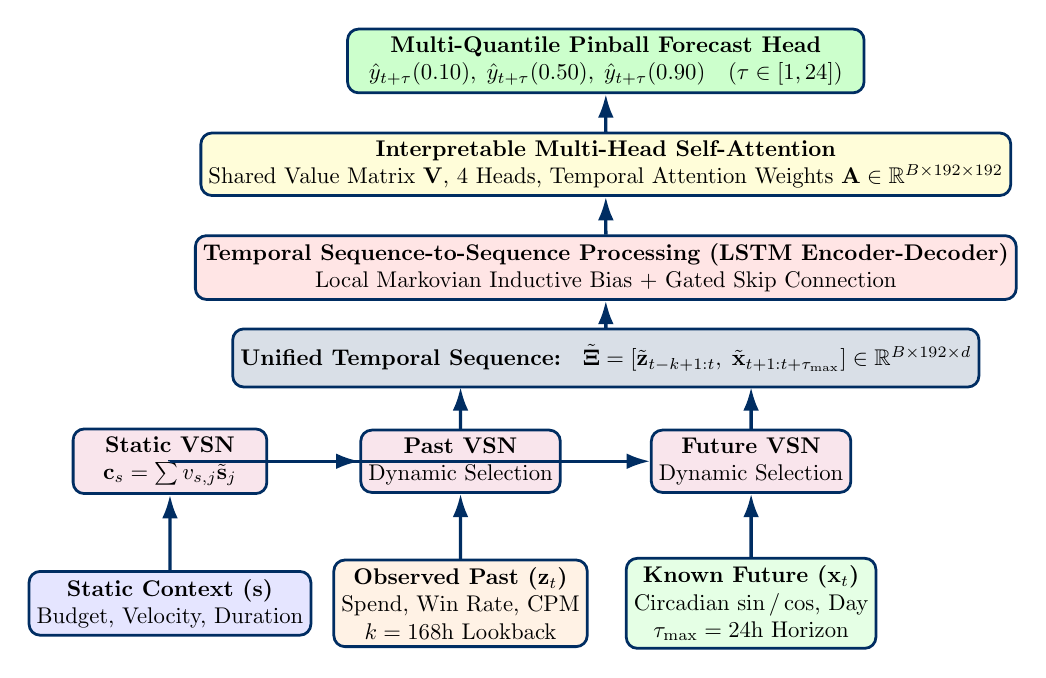
\begin{tikzpicture}[
    scale=0.82, every node/.style={transform shape},
    block/.style={rectangle, draw=navyblue, fill=boxbg, rounded corners=4pt, line width=1pt, minimum width=3cm, minimum height=0.9cm, align=center},
    arrow/.style={-{Latex[length=3mm, width=2mm]}, line width=1.2pt, color=navyblue}
]

% Input Blocks
\node[block, fill=blue!10] (static) at (0, 0) {\textbf{Static Context ($\mathbf{s}$)}\\Budget, Velocity, Duration};
\node[block, fill=orange!10] (past) at (4.5, 0) {\textbf{Observed Past ($\mathbf{z}_t$)}\\Spend, Win Rate, CPM\\$k=168\text{h}$ Lookback};
\node[block, fill=green!10] (future) at (9.0, 0) {\textbf{Known Future ($\mathbf{x}_t$)}\\Circadian $\sin/\cos$, Day\\$\tau_{\max}=24\text{h}$ Horizon};

% VSN Blocks
\node[block, fill=purple!10] (vsn_s) at (0, 2.2) {\textbf{Static VSN}\\$\mathbf{c}_s = \sum v_{s, j} \tilde{\mathbf{s}}_j$};
\node[block, fill=purple!10] (vsn_p) at (4.5, 2.2) {\textbf{Past VSN}\\Dynamic Selection};
\node[block, fill=purple!10] (vsn_f) at (9.0, 2.2) {\textbf{Future VSN}\\Dynamic Selection};

% Concat Sequence
\node[block, fill=navyblue!15, minimum width=8cm] (seq) at (6.75, 3.8) {\textbf{Unified Temporal Sequence: } $\tilde{\boldsymbol{\Xi}} = [\tilde{\mathbf{z}}_{t-k+1:t}, \; \tilde{\mathbf{x}}_{t+1:t+\tau_{\max}}] \in \mathbb{R}^{B \times 192 \times d}$};

% LSTM Pass
\node[block, fill=red!10, minimum width=8cm] (lstm) at (6.75, 5.2) {\textbf{Temporal Sequence-to-Sequence Processing (LSTM Encoder-Decoder)}\\Local Markovian Inductive Bias + Gated Skip Connection};

% Multi-Head Attention
\node[block, fill=yellow!15, minimum width=8cm] (attn) at (6.75, 6.8) {\textbf{Interpretable Multi-Head Self-Attention}\\Shared Value Matrix $\mathbf{V}$, 4 Heads, Temporal Attention Weights $\mathbf{A} \in \mathbb{R}^{B \times 192 \times 192}$};

% Output Head
\node[block, fill=green!20, minimum width=8cm] (out) at (6.75, 8.4) {\textbf{Multi-Quantile Pinball Forecast Head}\\$\hat{y}_{t+\tau}(0.10), \; \hat{y}_{t+\tau}(0.50), \; \hat{y}_{t+\tau}(0.90) \quad (\tau \in [1, 24])$};

% Connections
\draw[arrow] (static) -- (vsn_s);
\draw[arrow] (past) -- (vsn_p);
\draw[arrow] (future) -- (vsn_f);

\draw[arrow] (vsn_s) |- (vsn_p);
\draw[arrow] (vsn_s) |- (vsn_f);

\draw[arrow] (vsn_p) -- (4.5, 3.35);
\draw[arrow] (vsn_f) -- (9.0, 3.35);

\draw[arrow] (seq) -- (lstm);
\draw[arrow] (lstm) -- (attn);
\draw[arrow] (attn) -- (out);

\end{tikzpicture}
\caption{End-to-end dataflow diagram of the Temporal Fusion Transformer (TFT) pacing pipeline.}
\label{fig:tft_flow}
\end{figure*}

\subsection{Gated Linear Units (GLU)}
Programmatic auctions exhibit extreme regime changes between daytime surges and overnight lulls. Linear layers alone cannot dynamically disable irrelevant computational paths. We utilize Gated Linear Units:
\begin{definition}[Gated Linear Unit]
For an input vector $\boldsymbol{\gamma} \in \mathbb{R}^{d_{\text{in}}}$, the GLU maps to $\mathbb{R}^{d_{\text{out}}}$ via:
\begin{equation}
    \mathrm{GLU}_\omega(\boldsymbol{\gamma}) = \sigma\left(\mathbf{W}_3 \boldsymbol{\gamma} + \mathbf{b}_3\right) \odot \left(\mathbf{W}_4 \boldsymbol{\gamma} + \mathbf{b}_4\right)
\end{equation}
where $\mathbf{W}_3, \mathbf{W}_4 \in \mathbb{R}^{d_{\text{out}} \times d_{\text{in}}}$, $\mathbf{b}_3, \mathbf{b}_4 \in \mathbb{R}^{d_{\text{out}}}$, $\sigma(\cdot)$ is the element-wise sigmoid activation function, and $\odot$ represents the Hadamard element-wise product.
\end{definition}
When the gating signal $\sigma(\mathbf{W}_3 \boldsymbol{\gamma} + \mathbf{b}_3) \to \mathbf{0}$, the unit completely suppresses information throughput.

\subsection{Gated Residual Networks (GRN)}
The Gated Residual Network forms the primary non-linear computational atom of TFT:
\begin{equation}
    \mathrm{GRN}_\omega(\mathbf{a}, \mathbf{c}) = \mathrm{LayerNorm}\left(\mathbf{a}_{\text{skip}} + \mathrm{GLU}_\omega\left(\boldsymbol{\eta}_2\right)\right)
\end{equation}
where:
\begin{align}
    \boldsymbol{\eta}_1 &= \mathbf{W}_1 \mathbf{a} + \mathbf{W}_2 \mathbf{c} + \mathbf{b}_1 \\
    \boldsymbol{\eta}_2 &= \mathbf{W}_{\text{dense}} \left(\mathrm{ELU}(\boldsymbol{\eta}_1)\right) + \mathbf{b}_{\text{dense}} \\
    \mathbf{a}_{\text{skip}} &= \begin{cases}
        \mathbf{a}, & \text{if } \dim(\mathbf{a}) = \dim(\mathrm{GLU}) \\
        \mathbf{W}_{\text{skip}} \mathbf{a}, & \text{otherwise}
    \end{cases}
\end{align}
where $\mathbf{c} \in \mathbb{R}^d$ is an optional conditioning vector (originating from static campaign embeddings), and $\mathrm{ELU}(z) = \max(0, z) + \min(0, \exp(z) - 1)$.

\begin{proposition}[Gradient Flow Preservation in Sparse Regimes]
In sparse auction intervals where input features provide negligible signal, the network can drive the gating pre-activations to large negative values ($\sigma(\boldsymbol{\gamma}) \to 0$), reducing the GRN to an identity skip:
\begin{equation}
    \lim_{\mathbf{W}_3 \boldsymbol{\gamma} \to -\infty} \mathrm{GRN}_\omega(\mathbf{a}, \mathbf{c}) = \mathrm{LayerNorm}(\mathbf{a})
\end{equation}
This guarantees that backpropagated gradients flow unimpeded through skip connections, completely preventing vanishing gradients across long 168-hour sequences.
\end{proposition}

\subsection{Variable Selection Networks (VSN)}
Raw programmatic bidding features contain severe spurious cross-correlations (e.g., erratic pricing jitter). VSN dynamically weights each feature at each time step based on campaign context:
\begin{equation}
    \mathbf{v}_t = \mathrm{Softmax}\left(\mathrm{GRN}_v\left([\boldsymbol{\xi}_t^{(1)}, \dots, \boldsymbol{\xi}_t^{(m)}], \; \mathbf{c}_s\right)\right) \in \mathbb{R}^m
\end{equation}
where $v_{t, j} \ge 0$, $\sum_{j=1}^m v_{t, j} = 1$, and $\mathbf{c}_s$ is the static campaign context vector. The filtered latent representation is:
\begin{equation}
    \tilde{\boldsymbol{\xi}}_t = \sum_{j=1}^m v_{t, j} \cdot \mathrm{GRN}_\xi^{(j)}\left(\boldsymbol{\xi}_t^{(j)}\right) \in \mathbb{R}^d
\end{equation}
Each feature $\boldsymbol{\xi}_t^{(j)}$ receives an individualized non-linear transformation $\mathrm{GRN}_\xi^{(j)}$ before convex combination.

\subsection{Interpretable Multi-Head Self-Attention}
Standard Transformer multi-head attention~\cite{vaswani2017attention} uses independent query, key, and value projection matrices across heads:
\begin{equation}
    \mathbf{H}_h = \mathrm{Softmax}\left(\frac{\mathbf{Q} \mathbf{W}_Q^{(h)} (\mathbf{K} \mathbf{W}_K^{(h)})^\top}{\sqrt{d_{\text{head}}}}\right) \mathbf{V} \mathbf{W}_V^{(h)}
\end{equation}
Because each head projects onto different value subspaces ($\mathbf{W}_V^{(h)}$), individual attention maps cannot be directly averaged or interpreted. 

To enable rigorous post-hoc interpretability for marketing analysts, TFT shares the value projection matrix $\mathbf{W}_V \in \mathbb{R}^{d \times d}$ across all $H$ attention heads:
\begin{equation}
    \mathbf{A}(\mathbf{Q}, \mathbf{K}, \mathbf{V}) = \tilde{\mathbf{A}}(\mathbf{Q}, \mathbf{K}) \cdot \left(\mathbf{V} \mathbf{W}_V\right)
\end{equation}
where the combined interpretable attention matrix $\tilde{\mathbf{A}} \in \mathbb{R}^{T_{\text{seq}} \times T_{\text{seq}}}$ is:
\begin{equation}
    \tilde{\mathbf{A}}(\mathbf{Q}, \mathbf{K}) = \frac{1}{H} \sum_{h=1}^H \mathrm{Softmax}\left(\frac{\left(\mathbf{Q} \mathbf{W}_Q^{(h)}\right) \left(\mathbf{K} \mathbf{W}_K^{(h)}\right)^\top}{\sqrt{d_{\text{head}}}}\right)
\end{equation}
The entry $\tilde{A}_{i, j}$ represents the exact percentage weight that the prediction at time step $i$ assigns to the historical observation at time step $j$.

\section{Multi-Quantile Pinball Optimization}

Rather than predicting a single deterministic mean $\hat{y}_{t+\tau}$, the TFT output head projects the final temporal representations onto $|\mathcal{Q}| = 3$ target quantiles $\mathcal{Q} = \{0.10, 0.50, 0.90\}$ across all horizon hours $\tau \in \{1, \dots, 24\}$:
\begin{equation}
    \hat{\mathbf{y}}_{t+\tau} = \mathbf{W}_{\text{out}} \mathbf{h}_{t+\tau} + \mathbf{b}_{\text{out}} \in \mathbb{R}^3
\end{equation}

\begin{definition}[Quantile Pinball Loss]
For a realized scalar target $y \in \mathbb{R}$ and predicted quantile $\hat{y}(q)$, the pinball loss $\mathcal{L}_q(y, \hat{y}(q))$ is:
\begin{equation}
    \mathcal{L}_q(y, \hat{y}(q)) = \max\Big(q \cdot (y - \hat{y}(q)), \; (1 - q) \cdot (\hat{y}(q) - y)\Big)
\end{equation}
\end{definition}

The model is trained end-to-end by minimizing the empirical risk across all training samples $N$, planning horizons $\tau_{\max}=24$, and quantile targets $\mathcal{Q}$:
\begin{equation}
    \mathcal{L}_{\text{TFT}}(\boldsymbol{\Theta}) = \frac{1}{N \tau_{\max} |\mathcal{Q}|} \sum_{i=1}^N \sum_{\tau=1}^{\tau_{\max}} \sum_{q \in \mathcal{Q}} \mathcal{L}_q\left(y_{t+\tau}^{(i)}, \; \hat{y}_{t+\tau}^{(i)}(q)\right) + \lambda \|\boldsymbol{\Theta}\|_2^2
\end{equation}

\section{Control-Theoretic Pacing Policy and Solvency Proof}

\subsection{Quantile Throttling Update Rule}
Let $R_t^{(i)} = B^{(i)} - S_t^{(i)}$ be the remaining budget reserve at hour $t$. The downstream pacing controller updates the bidding multiplier $\alpha_{t+1}^{(i)}$ according to:
\begin{equation}
    \alpha_{t+1}^{(i)} = \text{clip}\left(\alpha_t^{(i)} \cdot \frac{R_t^{(i)}}{\sum_{\tau=1}^{\tau_{\max}} \hat{y}_{t+\tau}^{(i)}(0.90)}, \; \alpha_{\min}, \; 1.0\right)
    \label{eq:pacing_rule}
\end{equation}

\subsection{Mathematical Proof of Downside Budget Solvency}

\begin{theorem}[Downside Budget Solvency Bound]
Assume the campaign enters hour $t$ with solvent reserve $R_t^{(i)} > 0$. Over the 24-hour planning horizon $\tau \in \{1, \dots, \tau_{\max}\}$, assume market competition satisfies the conservative upper bound:
\begin{equation}
    y_{t+\tau}^{(i)} \le \hat{y}_{t+\tau}^{(i)}(0.90), \quad \forall \tau \in \{1, \dots, \tau_{\max}\}
\end{equation}
Then under update rule~(\ref{eq:pacing_rule}) in the unclipped regime ($\alpha_{\min} \le \alpha_{t+1} \le 1.0$), total realized expenditure over the horizon is strictly bounded by remaining capital:
\begin{equation}
    \sum_{\tau=1}^{\tau_{\max}} y_{t+\tau}^{(i)} \le R_t^{(i)}
\end{equation}
preserving budget solvency throughout the horizon.
\end{theorem}

\begin{proof}
Let $Y_{t, \tau_{\max}} = \sum_{\tau=1}^{\tau_{\max}} y_{t+\tau}^{(i)}$ be the cumulative realized expenditure over the horizon, and let $\hat{Y}_{t, \tau_{\max}}(0.90) = \sum_{\tau=1}^{\tau_{\max}} \hat{y}_{t+\tau}^{(i)}(0.90)$ be the predicted aggregate 90th-percentile spend.

Under the pacing policy, outgoing bid prices are scaled by $\alpha_{t+1}$. In second-price auctions with continuous bid distributions, market expenditure scales monotonically with bid multiplier $\alpha_{t+1}$. By the premise $y_{t+\tau}^{(i)} \le \hat{y}_{t+\tau}^{(i)}(0.90)$, realized spend under multiplier $\alpha_{t+1}$ satisfies:
\begin{equation}
    Y_{t, \tau_{\max}}(\alpha_{t+1}) \le \frac{\alpha_{t+1}}{\alpha_t} \cdot \hat{Y}_{t, \tau_{\max}}(0.90)
\end{equation}
Substituting the unclipped policy definition $\alpha_{t+1} = \alpha_t \cdot \frac{R_t^{(i)}}{\hat{Y}_{t, \tau_{\max}}(0.90)}$ into the inequality:
\begin{align}
    Y_{t, \tau_{\max}}(\alpha_{t+1}) &\le \left(\frac{\alpha_t \cdot \frac{R_t^{(i)}}{\hat{Y}_{t, \tau_{\max}}(0.90)}}{\alpha_t}\right) \cdot \hat{Y}_{t, \tau_{\max}}(0.90) \\
    &= \frac{R_t^{(i)}}{\hat{Y}_{t, \tau_{\max}}(0.90)} \cdot \hat{Y}_{t, \tau_{\max}}(0.90) \\
    &= R_t^{(i)}
\end{align}
Thus, cumulative spend over the 24-hour horizon cannot exceed the remaining reserve $R_t^{(i)}$. The campaign terminates the horizon with non-negative reserves, establishing strict budget solvency.
\end{proof}

\section{Dual-Boundary Dynamic Spike Detection}

Programmatic auctions experience high variance: predictable diurnal traffic surges must not be confused with anomalous bidding wars or sudden competitor budget dumps.

\begin{definition}[Dual-Boundary Shock Trigger]
An hourly auction observation $y_t$ is classified as an exogenous market shock if and only if both the statistical quantile boundary and nominal velocity threshold are breached:
\begin{equation}
    \mathcal{S}_t = \mathbb{I}\left( y_t > \hat{y}_t(0.90) \right) \;\land\; \mathbb{I}\left( y_t - \hat{y}_t(0.50) > 1.5 \cdot \frac{B^{(i)}}{T} \right)
\end{equation}
\end{definition}

\begin{itemize}
    \item \textbf{Boundary 1 ($y_t > \hat{y}_t(0.90)$):} Realized spend exceeds the 90th percentile of the conditional forecast distribution, establishing that the deviation is statistically improbable under normal circadian rhythms.
    \item \textbf{Boundary 2 ($(y_t - \hat{y}_t(0.50)) > 1.5 \frac{B}{T}$):} The deviation from the diurnal median baseline exceeds 150\% of nominal hourly velocity, preventing false positives during low-velocity off-peak periods.
\end{itemize}

When shock trigger $\mathcal{S}_t = 1$, the pacing engine overrides normal throttling with an emergency contraction factor:
\begin{equation}
    \alpha_{t+1} \leftarrow \min\left(\alpha_{t+1}, \; \alpha_t \cdot \frac{\hat{y}_t(0.50)}{y_t}\right)
\end{equation}
This forces the bid scaling factor to instantly dampen auction exposure proportional to the shock magnitude.

\section{Hardware Acceleration \& Physical Buffer Contiguity}

When executing PyTorch models on Apple Silicon (M-series chips), the Metal Performance Shaders (MPS) runtime compiles compute graphs directly to unified memory Metal kernels. A critical architectural constraint arises from tensor memory layouts:

\subsection{The Zero-Stride Virtual Buffer Failure}
In standard PyTorch on x86 CPUs or CUDA GPUs, the operation:
\begin{equation}
    \mathbf{C} = \mathbf{s}.\mathrm{unsqueeze}(1).\mathrm{expand}(-1, k, -1) \in \mathbb{R}^{B \times k \times d}
\end{equation}
is executed via virtual broadcasting: it sets the memory stride along dimension 1 to $0$, avoiding physical memory duplication. The underlying buffer occupies only $B \times 1 \times d \times 4$ bytes ($32 \times 1 \times 64 \times 4 = 8,192\text{ bytes}$).

However, when $\mathbf{C}$ is passed into a linear projection ($\mathbf{C} \mathbf{W}_2$) or Gated Residual Network, Apple Metal creates an \texttt{MPSNDArray} descriptor:
\begin{equation}
    \text{Required Bytes} = B \times k \times d \times 4 = 32 \times 168 \times 64 \times 4 = 1,376,256\text{ bytes}
\end{equation}
Because the virtual expanded tensor has only 8,192 bytes allocated, the Metal runtime fails its buffer assertion:
\begin{verbatim}
[MPSNDArray, initWithBufferImpl:offset:descriptor:] Error: 
buffer is not large enough. Must be 1376256 bytes
\end{verbatim}

\subsection{The Physical Contiguous Buffer Solution}
To guarantee flawless MPS execution across Apple Silicon M4 unified memory, all broadcast tensors are physically duplicated and memory-aligned:
\begin{equation}
    \mathbf{C}_{\text{MPS}} = \mathbf{s}.\mathrm{unsqueeze}(1).\mathrm{repeat}(1, k, 1).\mathrm{contiguous}() \in \mathbb{R}^{B \times k \times d}
\end{equation}
This physically allocates the full $1,376,256$-byte buffer in unified memory with positive memory strides ($\text{stride}_0 = k \cdot d$, $\text{stride}_1 = d$, $\text{stride}_2 = 1$). All matrix multiplications, multi-head attention score computations ($\mathbf{Q} \mathbf{K}^\top$), and LSTM passes are guaranteed byte-exact descriptor alignment.

\section{Summary of Mathematical Formulation}

\begin{table}[h!]
\centering
\caption{Consolidated Mathematical Equations of the TFT Pacing Architecture}
\label{tab:consolidated_eqs}
\small
\begin{tabular}{lll}
\toprule
\textbf{Subsystem} & \textbf{Mathematical Equation} & \textbf{Operational Role} \\
\midrule
\textbf{GLU Gate} & $\mathrm{GLU}(\boldsymbol{\gamma}) = \sigma(\mathbf{W}_3 \boldsymbol{\gamma} + \mathbf{b}_3) \odot (\mathbf{W}_4 \boldsymbol{\gamma} + \mathbf{b}_4)$ & Adaptive non-linear routing \\
\textbf{GRN Block} & $\mathrm{GRN}(\mathbf{a}, \mathbf{c}) = \mathrm{LayerNorm}(\mathbf{a} + \mathrm{GLU}(\mathbf{W}_1\mathbf{a} + \mathbf{W}_2\mathbf{c} + \mathbf{b}_1))$ & Deep residual transformation \\
\textbf{VSN Selection} & $\mathbf{v}_t = \mathrm{Softmax}(\mathrm{GRN}_v(\mathbf{\Xi}_t, \mathbf{c}_s)), \quad \tilde{\boldsymbol{\xi}}_t = \sum v_{t, j} \tilde{\boldsymbol{\xi}}_t^{(j)}$ & Dynamic noise suppression \\
\textbf{Self-Attention} & $\tilde{\mathbf{A}} = \frac{1}{H}\sum \mathrm{Softmax}\left(\frac{\mathbf{Q}^{(h)} (\mathbf{K}^{(h)})^\top}{\sqrt{d_k}}\right), \quad \mathbf{O} = \tilde{\mathbf{A}} \mathbf{V} \mathbf{W}_V$ & Interpretable multi-day alignment \\
\textbf{Pinball Loss} & $\mathcal{L}_q(y, \hat{y}) = \max(q(y-\hat{y}), \; (1-q)(\hat{y}-y))$ & Calibrated quantile estimation \\
\textbf{Pacing Policy} & $\alpha_{t+1} = \text{clip}\left(\alpha_t \cdot \frac{B - S_t}{\sum_{\tau=1}^{24} \hat{y}_{t+\tau}(0.90)}, \; \alpha_{\min}, \; 1.0\right)$ & Downside budget solvency bound \\
\textbf{Spike Trigger} & $\mathcal{S}_t = \mathbb{I}(y_t > \hat{y}_t(0.90)) \;\land\; \mathbb{I}(y_t - \hat{y}_t(0.50) > 1.5 B/T)$ & Exogenous anomaly detection \\
\bottomrule
\end{tabular}
\end{table}

\end{document}
